%%%%%%%%%%%%%%%%%%%%%%%%%%%%%%%%%%%%%%%%%
% M3 Presentation

%
%%%%%%%%%%%%%%%%%%%%%%%%%%%%%%%%%%%%%%%%%
%%% LINE 354
%To do:
%   Remove slide controls?
%   Photo of james and hasan, then repeat title slide

\documentclass[aspectratio=169]{beamer} %Remove for standard ppt slides. 

\usepackage[LGRgreek]{mathastext}


\usepackage{xcolor}
\usepackage{graphicx} % Allows including images
\usepackage{booktabs} % Allows the use of \toprule, \midrule and \bottomrule in tables
\usepackage{caption}
\usepackage{ragged2e} 
\usepackage{multirow}
\usepackage[font=small]{caption}
%\usepackage{cctbase, ccmap, CCTfntef}
\usepackage{wallpaper}
\usepackage{float}
\usepackage{amsmath}
\usepackage{listings}
\usepackage{tikz}
\usepackage{pgf-pie}
\usepackage{pgfplots} 
\usepackage[customcolors,beamer]{hf-tikz}

\usepackage{array}
\newcolumntype{P}[1]{>{\centering\arraybackslash}p{#1}}

\usetikzlibrary{calc}


%custom package for greek equation numbering : )
\usepackage{greekNumbers}

\makeatletter
\let\old@lstKV@SwitchCases\lstKV@SwitchCases
\def\lstKV@SwitchCases#1#2#3{}
\makeatother
\usepackage{lstlinebgrd}
\makeatletter
\let\lstKV@SwitchCases\old@lstKV@SwitchCases

\lst@Key{numbers}{none}{%
    \def\lst@PlaceNumber{\lst@linebgrd}%
    \lstKV@SwitchCases{#1}%
    {none:\\%
     left:\def\lst@PlaceNumber{\llap{\normalfont
                \lst@numberstyle{\thelstnumber}\kern\lst@numbersep}\lst@linebgrd}\\%
     right:\def\lst@PlaceNumber{\rlap{\normalfont
                \kern\linewidth \kern\lst@numbersep
                \lst@numberstyle{\thelstnumber}}\lst@linebgrd}%
    }{\PackageError{Listings}{Numbers #1 unknown}\@ehc}}

\renewrobustcmd{\beamer@@pause}[1][]{%
  \unless\ifmeasuring@%
  \ifblank{#1}%
    {\stepcounter{beamerpauses}}%
    {\setcounter{beamerpauses}{#1}}%
  \onslide<\value{beamerpauses}->\relax%
  \fi%
}

\makeatother



\definecolor{lbcolor}{rgb}{1.0,1.0,1.0}
\definecolor{ashgrey}{HTML}{E6E6E6}
\definecolor{armygreen}{rgb}{0.29, 0.33, 0.13}

\lstset{
	tabsize=4,
	rulecolor=,
	linewidth=0.95\linewidth,
	language=C,
        basicstyle=\tiny,
        upquote=false,
        aboveskip={1.5\baselineskip},
        columns=fixed,
        showstringspaces=false,
        extendedchars=true,
        breaklines=true,
        prebreak = \raisebox{0ex}[0ex][0ex]{\ensuremath{\hookleftarrow}},
        frame=single,
        showtabs=false,
        showspaces=false,
        showstringspaces=false,
        identifierstyle=\ttfamily,
        keywordstyle=,
        commentstyle=\color[rgb]{0.133,0.545,0.133},
        stringstyle=\color[rgb]{0.627,0.126,0.941},
        numbers=left,
        linebackgroundcolor={\ifodd\value{lstnumber}\color{ashgrey}\fi}
}

\graphicspath{ {images/} }

\setbeamertemplate{navigation symbols}{}

\definecolor{UBCblue}{rgb}{0.04706, 0.13725, 0.26667} % UBC Blue (primary)
\definecolor{UBCgrey}{rgb}{0.3686, 0.5255, 0.6235} % UBC Grey (secondary)
\definecolor{navy}{rgb}{0.0, 0.0, 0.5}
\definecolor{darkred}{rgb}{0.55, 0.0, 0.0}

%%Colour synonyms to help us know which colours are used where
\definecolor{titleBoxBackground}{named}{navy}
\definecolor{titleText}{named}{white}

\usetikzlibrary{decorations.pathreplacing,}
\tikzset{recurGenDiagram/.pic={
        code={

            \coordinate (base) at (3,0);
            \coordinate (root) at ($(base) + (0,1.5)$);
            
            
            \coordinate (male) at ($ (base) + (2,0) $);
            \coordinate (female) at ($ (base) + (2,3) $);
            \coordinate (ITMale) at ($ (male) + (4,1) $);
            \coordinate (RetailMale) at ($ (male) + (4,0) $);
            \coordinate (TradeMale) at ($ (male) + (4,-1) $);
            \coordinate (ITFemale) at ($ (female) + (4,1) $);
            \coordinate (RetailFemale) at ($ (female) + (4,0) $);
            \coordinate (TradeFemale) at ($ (female) + (4,-1) $);
            \coordinate (ellipsisSep) at (2.3,0);
            \coordinate (final) at ($(root) + (11.5,1)$);
            \coordinate (finalSep) at (-1,0);
            
        
            \draw [-latex](root) -- ($(male) + (-0.5,0)$);
            \draw [-latex](root) -- ($(female) + (-0.5,0)$);
            
            \draw [-latex]($(male) + (0.5,0)$) -- ($(ITMale) + (-0.5,0)$);
            \draw [-latex]($(male) + (0.5,0)$) -- ($(RetailMale) + (-0.5,0)$);
            \draw [-latex]($(male) + (0.5,0)$) -- ($(TradeMale) + (-0.5,0)$);
            
            \draw [-latex]($(female) + (0.5,0)$) -- ($(ITFemale) + (-0.5,0)$);
            \draw [-latex]($(female) + (0.5,0)$) -- ($(RetailFemale) + (-0.5,0)$);
            \draw [-latex]($(female) + (0.5,0)$) -- ($(TradeFemale) + (-0.5,0)$);                      


            \draw [] ($(ITMale) + (ellipsisSep) + (0.5,0)$) -- ($(final) + (finalSep)$);
            \draw [] ($(RetailMale) + (ellipsisSep) + (0.5,0)$) -- ($(final) + (finalSep)$);
            \draw [] ($(TradeMale) + (ellipsisSep) + (0.5,0)$) -- ($(final) + (finalSep)$);
            
            \draw [] ($(ITFemale) + (ellipsisSep) + (0.5,0)$) -- ($(final) + (finalSep)$);
            \draw [] ($(RetailFemale) + (ellipsisSep) + (0.5,0)$) -- ($(final) + (finalSep)$);
            \draw [] ($(TradeFemale) + (ellipsisSep) + (0.5,0)$) -- ($(final) + (finalSep)$);  


            \node[draw,text width=2cm] at ($(root) + (-1.5,0)$) {Population: \alert{1780424}};
            \node[text width=2cm] at ($(female) + (-1.3,-0.6)$) {48.8\%};
            \node[text width=2cm] at ($(male) + (-1.3,0.6)$) {51.2\%};

            \node[text width=2cm] at ($(ITFemale) + (-1.2,-0.1)$) {7.5\%};
            \node[text width=2cm] at ($(ITMale) + (-1.2,-0.1)$) {7.5\%};
            \node[text width=2cm] at ($(RetailFemale) + (-1.2,0.2)$) {9.5\%};
            \node[text width=2cm] at ($(RetailMale) + (-1.2,0.2)$) {9.5\%};
            \node[text width=2cm] at ($(TradeFemale) + (-1.2,0.15)$) {4.7\%};
            \node[text width=2cm] at ($(TradeMale) + (-1.2,0.15)$) {4.7\%};


            \node[text width=2cm] at ($(female) + (0.4,-1)$) {\alert{868847}};
            \node[text width=2cm] at ($(male) + (0.4,-1)$) {\alert{911577}};
            
            \node[text width=2cm] at ($(ITFemale) + (1.5,0)$) {\alert{65164}};
            \node[text width=2cm] at ($(ITMale) + (1.5,0)$) {\alert{68368}};
            \node[text width=2cm] at ($(RetailFemale) + (1.5,0)$) {\alert{82540}};
            \node[text width=2cm] at ($(RetailMale) + (1.5,0)$) {\alert{86600}};
            \node[text width=2cm] at ($(TradeFemale) + (1.5,0)$) {\alert{40836}};
            \node[text width=2cm] at ($(TradeMale) + (1.5,0)$) {\alert{42844}};            
            
            

            
            
            \node[inner sep=0pt] at (female) {
\includegraphics[width=0.1\textwidth]{images/Icons/girl.png}};
            \node[inner sep=0pt] at (male) {
\includegraphics[width=0.1\textwidth]{images/Icons/standing-up-man-.png}};
            
            \node[inner sep=0pt] at (ITMale) {
\includegraphics[width=0.05\textwidth]{images/Icons/it.png}};
            \node[inner sep=0pt] at (RetailMale) {
\includegraphics[width=0.05\textwidth]{images/Icons/shop.png}};
            \node[inner sep=0pt] at (TradeMale) {
\includegraphics[width=0.05\textwidth]{images/Icons/trading.png}};    

            \node[inner sep=0pt] at (ITFemale) {
\includegraphics[width=0.05\textwidth]{images/Icons/it.png}};
            \node[inner sep=0pt] at (RetailFemale) {
\includegraphics[width=0.05\textwidth]{images/Icons/shop.png}};
            \node[inner sep=0pt] at (TradeFemale) {
\includegraphics[width=0.05\textwidth]{images/Icons/trading.png}};
            
            \node[inner sep=0pt] at ($(RetailFemale)+(ellipsisSep)$) {
\includegraphics[width=0.05\textwidth]{images/Icons/more.png}};
            \node[inner sep=0pt] at ($(RetailMale)+(ellipsisSep)$) {
\includegraphics[width=0.05\textwidth]{images/Icons/more.png}};
            \node[inner sep=0pt] at ($(ITFemale)+(ellipsisSep)$) {
\includegraphics[width=0.05\textwidth]{images/Icons/more.png}};
            \node[inner sep=0pt] at ($(TradeMale)+(ellipsisSep)$) {
\includegraphics[width=0.05\textwidth]{images/Icons/more.png}}; 
            \node[inner sep=0pt] at ($(TradeFemale)+(ellipsisSep)$) {
\includegraphics[width=0.05\textwidth]{images/Icons/more.png}};
            \node[inner sep=0pt] at ($(ITMale)+(ellipsisSep)$) {
\includegraphics[width=0.05\textwidth]{images/Icons/more.png}};              

            \node[inner sep=0pt] at ($(ITFemale)+(ellipsisSep)+(0,0.5)$) {\scriptsize(All Characteristics)}; 

            \node[inner sep=0pt] at ($(TradeMale)+(0,-0.5)$) {
\includegraphics[width=0.05\textwidth]{images/Icons/more.png}};
            \node[inner sep=0pt] at ($(TradeFemale)+(0,-0.5)$) {
\includegraphics[width=0.05\textwidth]{images/Icons/more.png}};              
                    
            
            
            \node[draw,text width=1.4cm] at (final) {Apply Model 2};
            
            \draw [-latex]($(final) + (0,-0.5)$) -- ($(final) + (0,-1.0)$);                      
            \node[text width=2cm] at ($(final) + (0,-1.5)$) {$$\sum_{People}$$};
            
            \draw [-latex]($(final) + (0,-2.3)$) -- ($(final) + (0,-3.0)$);                      
            \node[text width=2cm] at ($(final) + (0.5,-3.5)$) {\large To \%};
            
  }}
}

 \tikzset{
    invisible/.style={opacity=0},
    visible on/.style={alt={#1{}{invisible}}},
    alt/.code args={<#1>#2#3}{%
      \alt<#1>{\pgfkeysalso{#2}}{\pgfkeysalso{#3}} % \pgfkeysalso doesn't change the path
    },
  }

\newcommand{\tikzmarkA}[1]{\tikz[overlay,remember picture] \node (#1) {};}

\newcommand<>{\LabelText}[4]{%
    \tikzmarkA{a}#1\tikzmarkA{b}%
    \begin{tikzpicture}[overlay,remember picture]
        \path (a.north) -- (b.north) node [yshift=#4, midway,rectangle,draw=#3,line width=1.5pt,rounded corners=2pt,inner sep=2pt]  (label) {\textbf{\small #2}\strut};
        \draw [thick,-stealth,shorten >=5pt,#3] (label.south) -- ($(a.north)!0.5!(b.north)$);
    \end{tikzpicture}%
}

\pgfplotsset{compat=1.18} 

\mode<presentation> {

\useinnertheme[shadow=true]{rounded}
\useoutertheme{infolines}
\usecolortheme{wolverine}
%\usecolortheme{albatross}
\setbeamerfont{block title}{size={}}
%\usefonttheme{serif} 

%Main title colour on the homepage
\setbeamercolor{titlelike}{parent=structure,fg=titleText,bg=titleBoxBackground!85!titleText}
\setbeamercolor{title}{fg=titleText}
%Titles on every page
\setbeamercolor{frametitle}{bg=navy,fg=titleText}
\setbeamercolor{block title}{bg=red!70,fg=white}
\setbeamercolor{block title alerted}{bg=navy!70,fg=white}
\setbeamercolor{subsectionTitleBoxes}{bg=UBCgrey,fg=white}


%Colour palette - it is possible to mix and match colours for the different tiles at the top and bottom.
\setbeamercolor{palette primary}{bg=navy,fg=white} %Top right tile and bottom right tile.
\setbeamercolor{palette secondary}{bg=UBCgrey,fg=white} %Middle tile at the bottom
\setbeamercolor{palette tertiary}{bg=red,fg=white} %Top left tile and bottom left tile 
\setbeamercolor{palette quaternary}{bg=UBCgrey,fg=white}
\setbeamercolor{structure}{fg=UBCblue} % itemize, enumerate, etc
\setbeamercolor{section in toc}{fg=UBCblue} % Table of contents sections

\setbeamercolor{local structure}{fg=darkred}
\setbeamertemplate{enumerate item}[square]



%\usecolortheme{albatross}
%\usecolortheme{beaver}
%\usecolortheme{beetle}
%\usecolortheme{crane}
%\usecolortheme{dolphin}
%\usecolortheme{dove}
%\usecolortheme{fly}
%\usecolortheme{lily}
%\usecolortheme{orchid}
%\usecolortheme{rose}
%\usecolortheme{seagull}
%\usecolortheme{seahorse}
%\usecolortheme{whale}
%\usecolortheme{wolverine}


}



%
%----------------------------------------------------------------------------------------
%	TITLE PAGE
%----------------------------------------------------------------------------------------

\title[\sffamily Remote Work: \textit{Fad or Future?}]{Remote Work: \textit{Fad or Future?}} % The short title appears at the bottom of every slide, the full title is only on the title page

\author{\sffamily{Team 15440}} % Your name
\institute[\sffamily{WBGS}] % Your institution as it will appear on the bottom of every slide, may be shorthand to save space
{
Hamish Starling, Hasan Shahrestani, Luke Powney, James Elcock \\
\vskip 0.5em
\textbf{Watford Boys Grammar School}
\\ % Your institution for the title page
%\medskip
 % Your email address
%\textit{123456@erau.edu\\}
%\normalsize\textit{Tuesday, March 28, 2017\\IEEE West Virginia Section}
}
\titlegraphic{
\includegraphics[scale =0.4]{images/UkFlag.png} % Example - can be changed.
%\includegraphics[scale = 0.2]{Figures/LOGO/ERAU_logo.pdf}
}
\date[\sffamily April 25th 2022]{April 25th 2022} 



% Date, can be changed to a custom date

\begin{document}

\begin{frame}
\titlepage % Print the title page as the first slide

\end{frame}


\setbeamertemplate{section in toc}[square] %Changes how the numbered points on the table of contents are displayed.
\begin{frame}
\frametitle{Overview} % Table of contents slide, comment this block out to remove it
%\tableofcontents % Throughout your presentation, if you choose to use \section{} and \subsection{} commands, these will automatically be printed on this slide as an overview of your presentation
% This takes the place of the executive summary in the original report. Could we leave our methods out and just describe the problems? Don't know
\vskip -1em
\begin{columns}[T]
  \onslide<1-> {\begin{column}{0.33\textwidth}
    \begin{center}
    \footnotesize\textbf{Part I:\\ Ready or Not}
    \end{center}
    {\footnotesize\color[named]{navy}{\textbf{Problem}}}
    \begin{itemize}
        \footnotesize
        \item[$\rightarrow$] Percentage of remote ready jobs in 5 given cities.
        %$$\Downarrow$$
    \end{itemize}
    
  \end{column}}


    \begin{column}{.01\textwidth}
        %\rule{.1mm}{0.375\textheight}
    \end{column}
    
  \onslide<2->{
  \begin{column}{0.33\textwidth}
      \begin{center}
    \footnotesize\textbf{Part II:\\ Remote Control}
    \end{center}
      

    {\footnotesize\color[named]{navy}{\textbf{Problem}}}
    \begin{itemize}
        \footnotesize
        \item[$\rightarrow$] Will a given remote-ready worker \textit{actually} work from home?
        %$$\Downarrow$$
    \end{itemize}
      
  \end{column} }

    \begin{column}{.01\textwidth}
        %\rule{.1mm}{0.375\textheight}
    \end{column}
  
  \onslide<3-> {\begin{column}{0.33\textwidth}
      \begin{center}
    \footnotesize\textbf{Part III: \\ Just a Little Home-Work}
    \end{center}
    
    {\footnotesize\color[named]{navy}{\textbf{Problem}}}
    \begin{itemize}
        \footnotesize
        \item[$\rightarrow$] Determine true remote worker percentage in each city.
        \item[$\rightarrow$] Rank WFH's impact on the 5 cities.
        %$$\Downarrow$$
    \end{itemize}

  \end{column}  }
\end{columns}

\vskip 2em

\begin{columns}[T]
  \onslide<1-> {\begin{column}{0.33\textwidth}
    {\footnotesize\color[named]{red}{\textbf{Approach}}}    
    \begin{itemize}        \footnotesize
%        \item[$\rightarrow$] Sector by sector regression for changing industry share in each city, applied to industry percentages.
        \item[$\rightarrow$] Exponential regression on industries; percentage in each industry.        
    \end{itemize}
  \end{column}}

    \begin{column}{.01\textwidth}
        %\rule{.1mm}{0.375\textheight}
    \end{column}
    
  \onslide<2-> {\begin{column}{0.33\textwidth}
    {\footnotesize\color[named]{red}{\textbf{Approach}}}    
    \begin{itemize}        \footnotesize
%        \item[$\rightarrow$] Demographic factors fed into a conditional probability model for percentage chance.
        \item[$\rightarrow$] Conditional probability on demographic factors        
    \end{itemize}      
      
  \end{column}}
  
    \begin{column}{.01\textwidth}
        %\rule{.1mm}{0.375\textheight}
    \end{column}
  \onslide<3-> {  
  \begin{column}{0.33\textwidth}
    {\footnotesize\color[named]{red}{\textbf{Approach}}}    
    \begin{itemize}        \footnotesize
%        \item[$\rightarrow$] Population Simulation Method to apply Part II model over simulated population generated from Part I industry projections. 
        \item[$\rightarrow$] Population Simulation Method combining models I and II.
    \end{itemize}     
    

  \end{column}  }
\end{columns}


 

\end{frame}

	%------------------------------------------------
\section{Introduction}

\subsection{Global Assumptions}
\begin{frame}{Global Assumption}
     \textbf{G.1:}     ``Working from home" is a general term including partial and full remote work.
        
            %\textit{The problems do not specify how to deal with partial and full working from home; we don't want to exclude either, but separating them adds complexity for little gain.

\end{frame}

%\begin{frame}
%\begin{figure}
%	\includegraphics[width=2in,height= 2in]{Figures/LOGO/Updated-eagle-01-TM.eps}
%\end{figure}
%\end{frame}


%------------------------------------------------

%\begin{frame}
%\begin{figure}
%	\centering
%	\includegraphics[scale=0.3]{Figures/LOGO/er-logo-1970s-1.jpg}
%\end{figure}
%\end{frame}

%------------------------------------------------

\newcommand{\sectionheader}{
    \begin{frame}
      \vfill
      \centering
      \begin{beamercolorbox}[sep=8pt,center,shadow=false,rounded=true]{subsectionTitleBoxes}
        \usebeamerfont{title}\insertsectionhead\par%
      \end{beamercolorbox}
      \vfill
    \end{frame}
}


\section{Part I: Ready or Not}
    \sectionheader
    
    \subsection{Problem Statement}
        \begin{frame}{Problem Statement}
        \textbf{Given Problem}
        
        \begin{itemize}
            \item[$\rightarrow$] Create a model which, for a given city, estimates the percentage of workers whose jobs are currently remote-ready. The model should be applied to the following cities:
        \end{itemize}
           
               \hfil \textbf{Seattle}
               \hfil \textbf{Omaha}
               \hfil \textbf{Scranton}
               \hfil \textbf{Liverpool}
               \hfil \textbf{Barry}
               \hfil
           
           
           \begin{figure}[H]
                  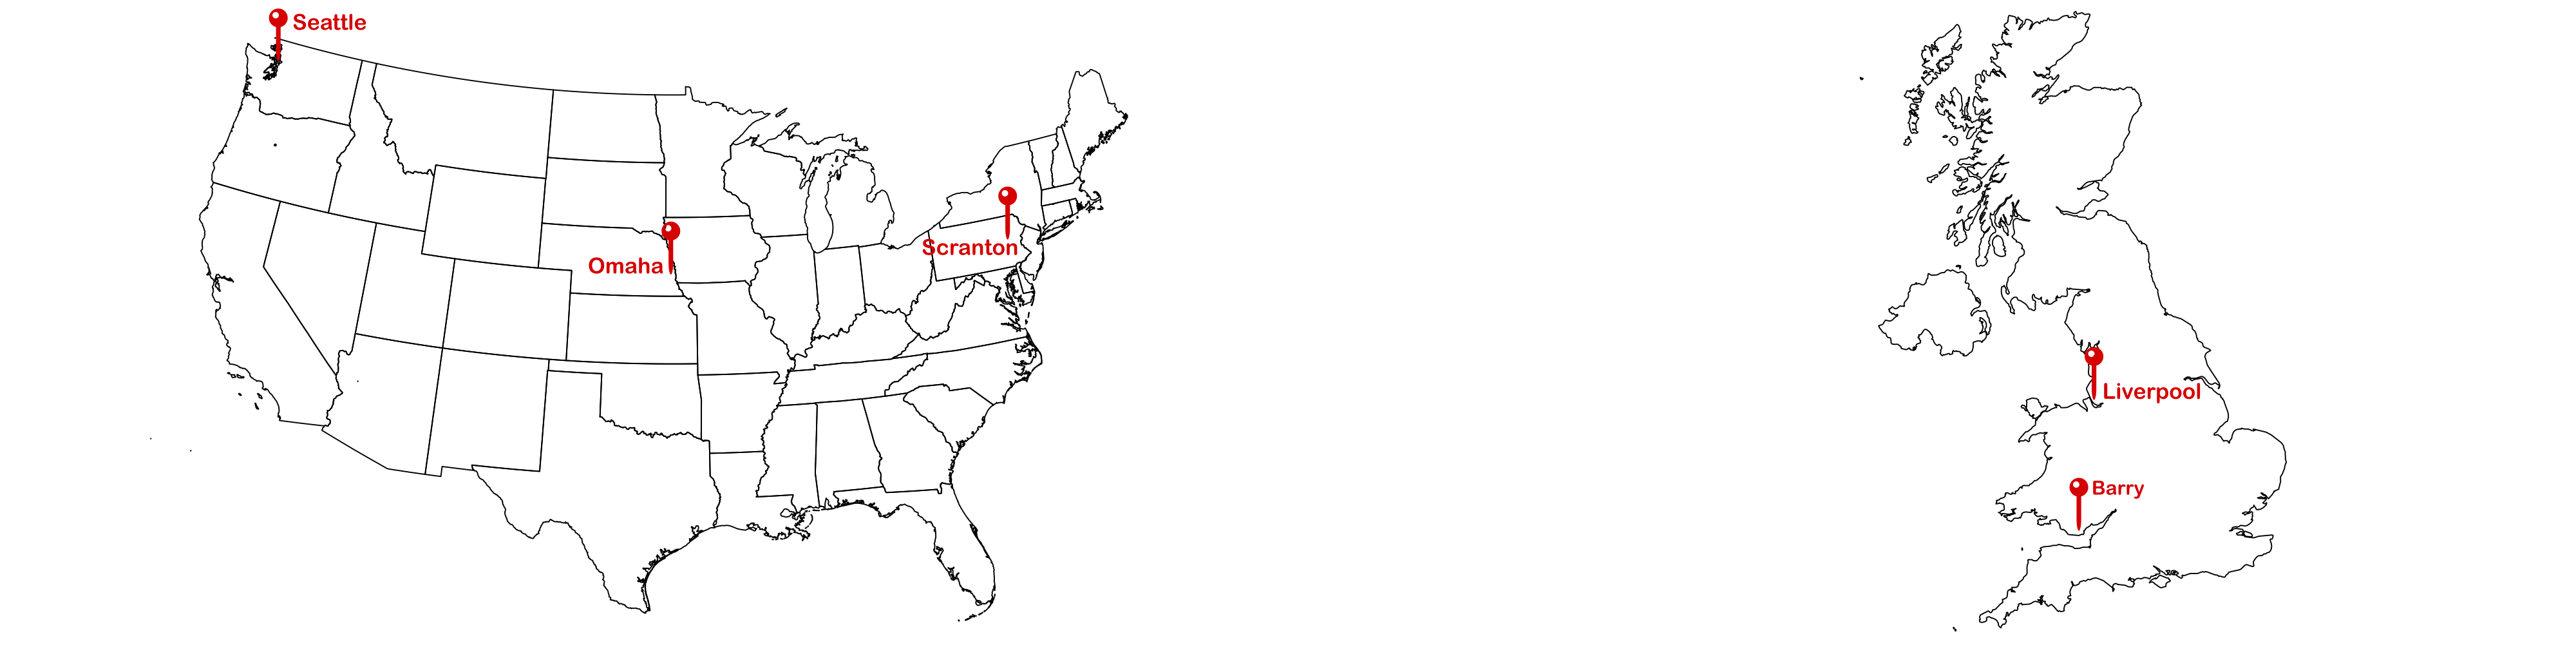
\includegraphics[height=0.5\textheight]{images/map.png}
                  
                \end{figure}
           %we could add a coat of arms / flag for each city underneath if you want. Don't know if that would look nice or a bit tacky.
           
    \end{frame}
        
            
    
    \subsection{Assumptions}
        \begin{frame}{Assumptions} \relax
         {\setlength{\leftmargini}{0.5cm}

            \begin{tikzpicture}
            \node[draw,text width=6cm,anchor=north west,visible on=<1->] at (0,4) {\vskip -0.6em \begin{enumerate} \item \alert{Remote Work Rate Constant} within industries over time.\end{enumerate}                 \begin{center}
                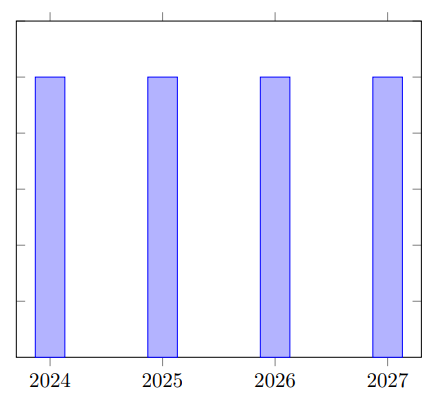
\includegraphics[height=0.4\textheight]{images/barchart.png}
            \end{center}};

      % 

            
            \node[draw,text width=6cm,anchor=north west,visible on=<2->] at (8,4) {\vskip -0.6em \begin{enumerate}  \setcounter{enumi}{1} \item \alert{Post-Pandemic Economy} \end{enumerate} 
                \begin{center}
                     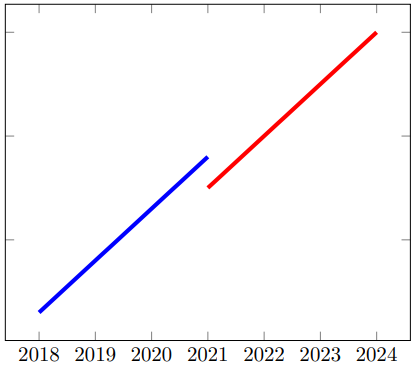
\includegraphics[height=0.4\textheight]{images/linegraph.png}
                \end{center}
            Pre-Pandemic trends in sector \\ workforce share, from lower base of post pandemic levels.};
            \node[draw,text width=6cm,anchor=north west,visible on=<3->] at (0,-1) {\vskip -0.6em \begin{enumerate} \setcounter{enumi}{2} \item \alert{Profession Only} - ``Remote \\ readiness" defined by job; not\\ employee.\end{enumerate}};
            \end{tikzpicture}       
        }
        \end{frame}    
    \subsection{Feature Identification}
        \begin{frame}{Variables \& Constants}
      
            \subsubsection{Table of Variables/Constants}
                % To summarise all of the choices made.
                % All tables should have a title, a header, a label, and a caption.
                
                \bgroup
                    \def\arraystretch{1.7}%  1 is the default
                \footnotesize \begin{table}[h!]
                  \begin{center}
                    %\label{tab:variables1} % U%e this to create a label for the table so you can later reference it with \ref
                    \begin{tabular}{|c|c|p{8cm}|c|} % Defines where vertical lines appear and the column alignment left centre or right
                      \hline 
                       \textbf{Type} & \textbf{Symbol} & \textbf{Definition} & \textbf{Units} \\ \hline
                
                Variable & $t$ & Time since 2000. & years\\ 
                Variable & $N_{I,C}(t)$ & Number of workers in industry I in city C at time t. & 1000 people  \\ % & used to separate cells in a row; \\ used to separate rows.
                Variable & $P_{I,C}(t)$ & Proportion of city C's jobs being in industry I at time t. & \% \\
                \color[named]{red}{Variable} & \color[named]{red}{$R_C(t)$} & {\textcolor [named] {red} {Percentage of city C's jobs being remote ready at time t.}} & \color[named]{red}{\%} \\
                Constant & $H_{I}$ & Proportion of remote ready jobs in a given industry I. & \% \\ 
                \hline
                
                    \end{tabular}
                    
                  \end{center}
                \end{table}
                \egroup            
            
        \end{frame}    
    \subsection{Developing the Model}
    
        \begin{frame}{Model Development}
            \begin{equation*}
                R_C(t) = \sum_I\ [P_{I,C}(t)\cdot H_I]     
            \end{equation*}
            \begin{figure}[H]
                  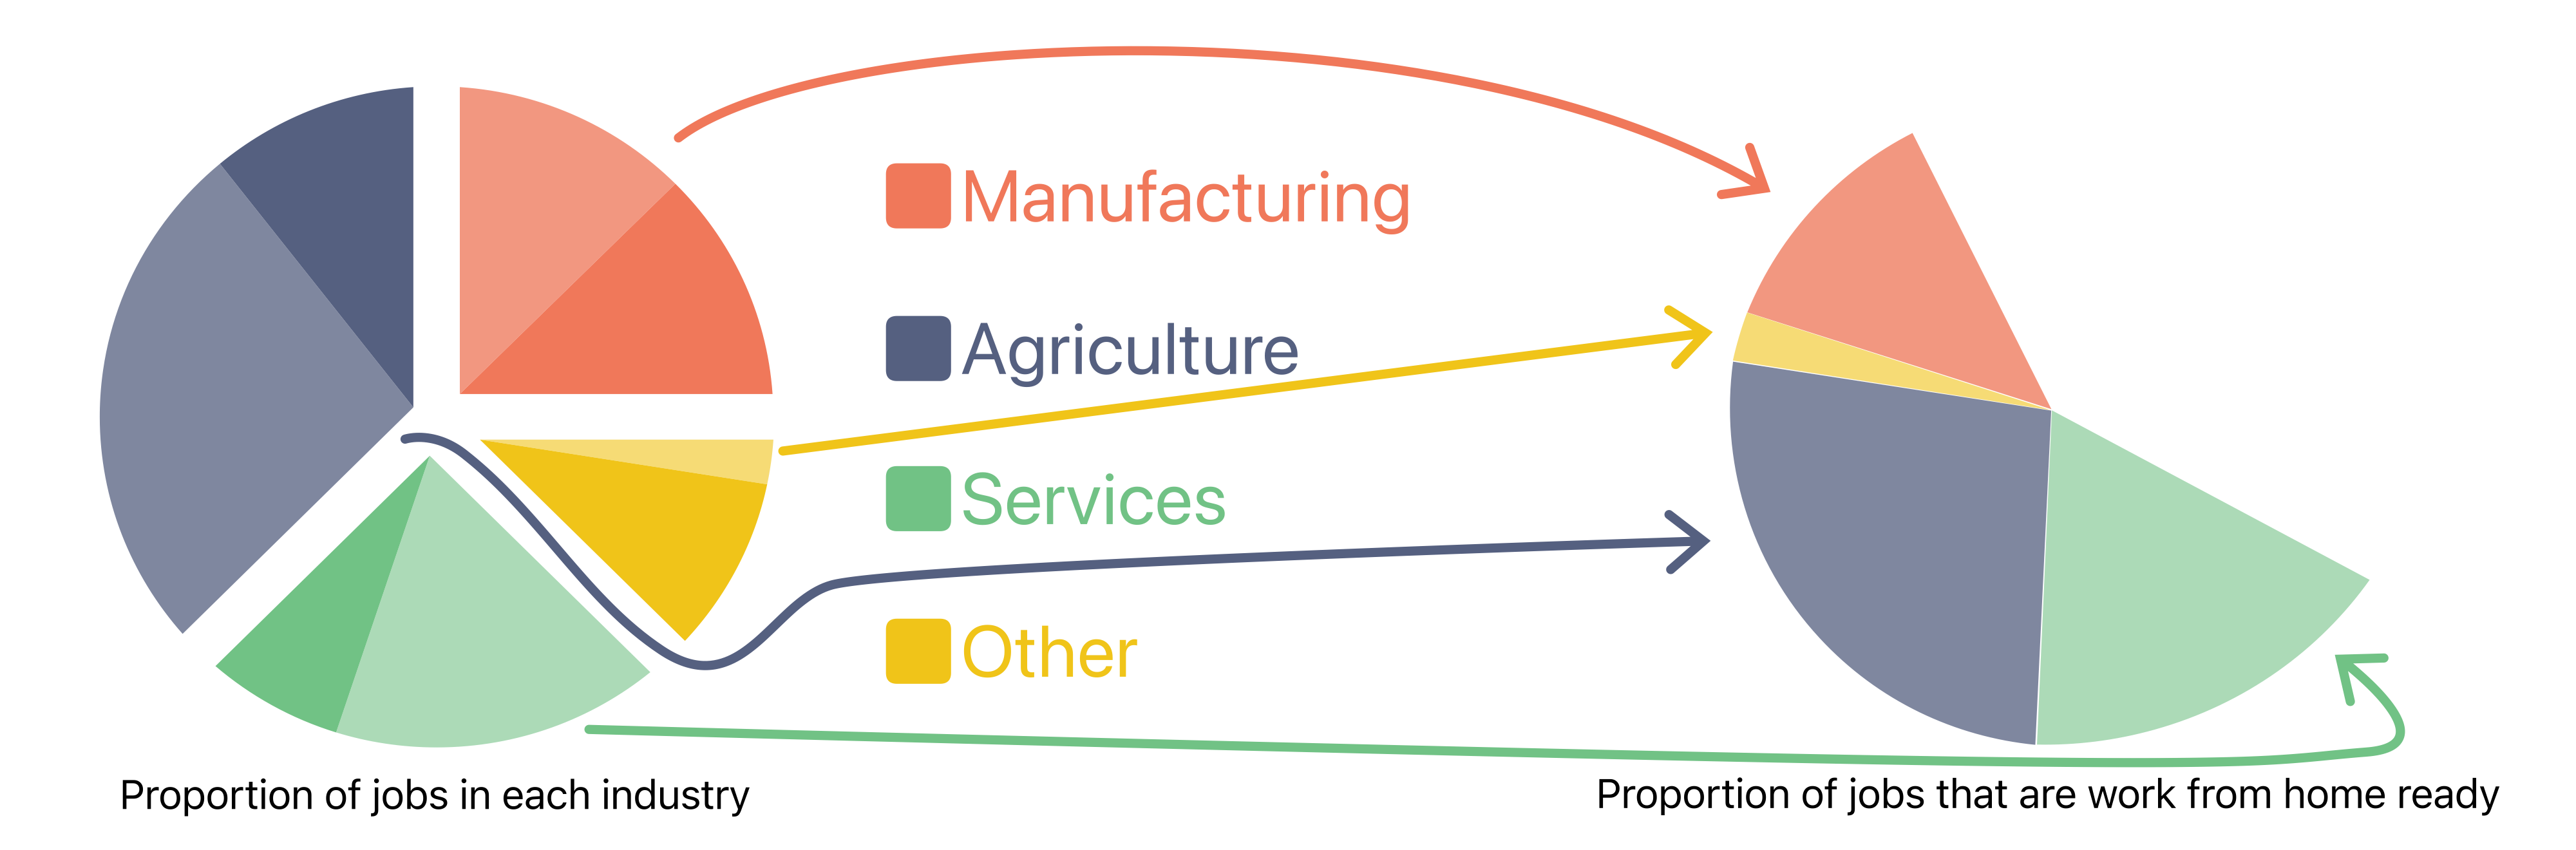
\includegraphics[height=0.60\textheight]{images/pie2.png}
                  
                \end{figure}
                \footnotetext[1]{Chart for intuition only; not real data!}
    
        \end{frame}    
        
        \begin{frame}{Finding Industry Trends}
                \begin{equation*}
                    \boxed{P_{I,C}(t) = a \cdot e^{b t}} %\tag{$\alpha$}}
                \end{equation*}
                
                \textbf{Justifications}
                \begin{itemize}
%                    \itemsep 0.5em
                    \item An exponential model better \textbf{fits the data}. \textit{Visually \& Mathematically (measuring PMCC of the data after logged)}
                    \pause
                    \item An exponential model demonstrates \textbf{asymptotic behaviour}.
                    \item Exponentials are established to represent \textbf{changes in populations} over time.
                    %Here you can mention that the you mean mathematically the PMCC of a logarithmic graph was very close to 1 for example Liverpool Education was -0.96 and Seattle Manufacturing was -0.95
                \end{itemize}  
            \footnotetext[1]{ $P_{I,C}$ - Proportion of city C's jobs being in industry I at time t.}
            \footnotetext[2]{ $a$,b are constants fitted to the data}
        \end{frame}    
  
    
                     
        \begin{frame}{$P_{I,C}(t)$ Exponential Regression}
            \vskip -1.5em  
            \begin{columns}[T]
                \begin{column}{0.75\linewidth}
                    \begin{figure}[H]
                      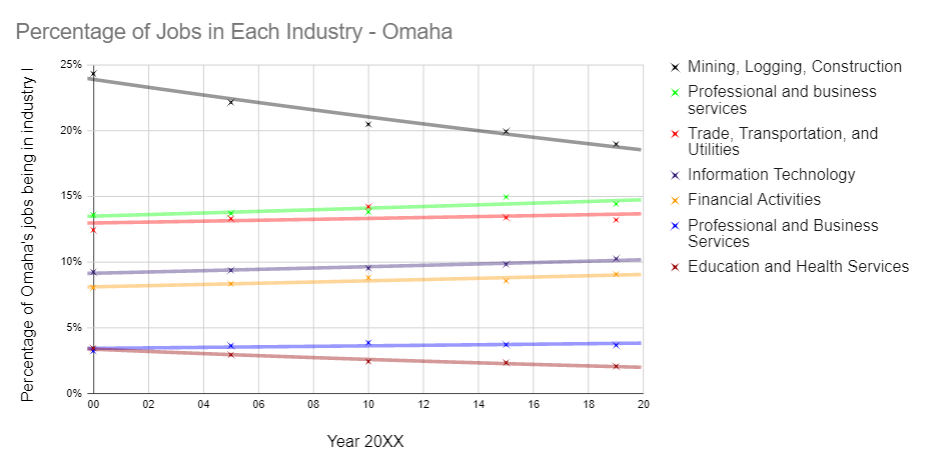
\includegraphics[height=0.7\textheight]{images/Omaha.png}
                      \caption{\scriptsize $P_{I,C}(t)$ vs $t$ with exponential trend lines; some industries omitted for clarity.}
                      \label{fig:chart3}
                    \end{figure}                    
                \end{column}
                \begin{column}{0.25\linewidth}
                    \scriptsize \begin{equation*}
                        \boxed{R_C(t) = \sum_I\ [\tikzmarkin<1>[set fill color=yellow,set border color=yellow]{z99}P_{I,C}(t)\tikzmarkend{z99}\cdot \tikzmarkin<2>[set fill color=yellow,set border color=yellow]{z100}H_I\tikzmarkend{z100}]}   
                    \end{equation*}
                \end{column}
            \end{columns}

                
                            
        \footnotetext[1]{Note: All jobs; not just remote ready ones.}
        \end{frame}  

        %\begin{frame}{Model Reminder}
        %    \begin{equation*}
        %        R_C(t) = \sum_I\ [P_{I,C}(t)\cdot H_I]     
        %   \end{equation*}
        %\end{frame}    
        
        \begin{frame}{The $H_{I}$ constant}
            \begin{itemize}
                \item $P_{I,C}(t)$ industries don't perfectly match given $H_{I}$ values' industries.\\ \hskip 1em $\implies$ weighted average where necessary
            \end{itemize}

            \vskip 0.7em
           \scriptsize \begin{table}[h!]
              \begin{center}
                \label{tab:HI} % Use this to create a label for the table so you can later reference it with \ref
                              
                \bgroup

                \def\arraystretch{1.5}%  1 is the default
                \begin{tabular}{|p{4.5cm}|p{6cm}|c|c|} % Defines where vertical lines appear and the column alignment left centre or right
                      \hline 
                       \textbf{$P_{I,C}(t)$ Industry} & \textbf{Given $H_I$ industry values}  & \textbf{Weights} & \textbf{$H_I$}\\
                      \hline 
                       Education and Health Services & Education / Health Services & 0.3 / 0.7 & 34\%\\
                       %Financial activities& Business and Financial Operations & - & 88\%\\
                       %Government & Legal / Office and Administrative / Management& 0.2 / 0.7 / 0.1 & 74\%\\
%                       Manufacturing& Production & - & 1\%\\
 %                      Mining, Logging, Construction & Trade, Transportation, and Utilities & - & 0\%\\
%                       Other services & - & - & 50\%\\
                       Professional and Business Services & Sales / Office and Administrative / Management & 0.5 / 0.4 / 0.1 & 49\%\\
%                       Trade, Transportation, and Utilities& Transportation and Material Moving & - & 30\%\\
                       Information Technology & Computer and Mathematical & - & 100\%\\
                       Leisure and Hospitality& Food Preparation and Service Related&- & 0\%\\
                       ... & ... & ... & ... \\
                     
                       
                      \hline 
                    \end{tabular}      
                \egroup                      
                    
                    \end{center}
                \end{table}
 %       \footnotetext[1]{
  %      Number of health and care workers in England and Wales for 2019 and 2020, UK-Gov, 2021 \\
   %     \hskip 1.95em School workforce in England, UK-Gov, 2020}
        \footnotetext[1]{$H_I$ is the percentage of jobs in industry I being remote ready.}
        \end{frame}    



                
    \subsection{Applying the Model}
        \begin{frame}{Results}
            
            \begin{columns}
            
                \begin{column}{0.48\linewidth}
                    \vskip 0.5em

                    {\centering\textbf{Example Regression for Industry Labour Market Share}}
                    \begin{align*}
                        &P_{trade,Omaha}(t) = 0.237\cdot e^{-0.0117t} \\
                        &P_{trade,Omaha}(24) = 17.90\ \% \\
                        &P_{trade,Omaha}(27) = 17.28\ \% \\
                    \end{align*}
                    \pause
                    \vskip -1.0em Then we multiply by $H_I$ ... \\ \vskip 1.0em
                    
                    \textbf{Model Reminder}
                    \begin{equation*}
                    R_C(t) = \sum_I\ [P_{I,C}(t)\cdot H_I]                             %\tag{$\dagger$}
                    \end{equation*}
                    \pause

                    
                % \begin{figure}[H]
                %   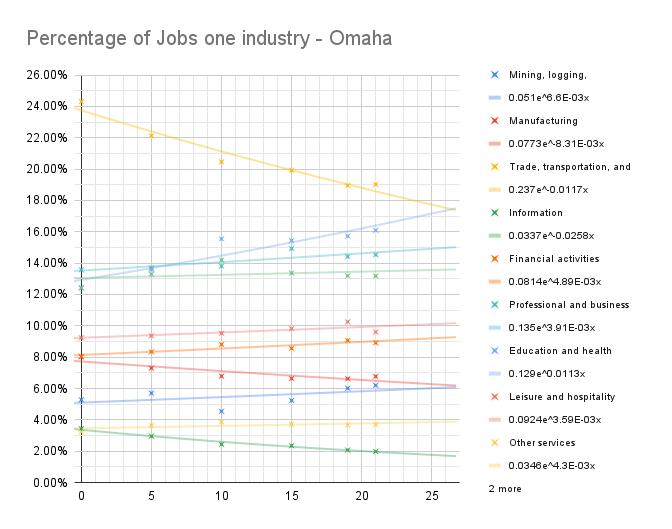
\includegraphics[width=\linewidth]{images/BEAB97A6-07C9-45F9-8B49-E371557909FE.png}
                %   \caption{$P_{I,C}(t)$ vs $t$ with exponential trend line}
                %   \label{fig:chart3}
                % \end{figure}
                
                \end{column}
                \begin{column}{0.48\linewidth}

                    \begin{table}[h!]
                      \begin{center}
                        \label{tab:results1} % Use this to create a label for the table so you can later reference it with \ref
                      
                        \begin{tabular}{|c|c|c|} % Defines where vertical lines appear and the column alignment left centre or right
                          \toprule 
                          \textbf{City} & \textbf{2024}  & \textbf{ 2027} \\
                          \midrule 
                          Seattle & 41\% & 42\% \\ 
                          Omaha & 40\% & 40\% \\ 
                          Barry & 39\% & 39\% \\ 
                          Scranton & 36\% & 36\% \\  
                          Liverpool & 31\% & 31\% \\  
                        \bottomrule 
                           
                        \end{tabular}
                          \caption{Percentage of jobs being remote ready.}                
                        
                      \end{center}
                    \end{table}
                \end{column}
            \end{columns}
        \end{frame}        
    \subsection{Evaluating the Model}
        \begin{frame}{Evaluation}
            \begin{itemize}
                \item[\textcolor{armygreen}{\textbf{+}}] Consistent with recent studies\footnotemark[1] suggesting 36 \% on average.
                \pause
                \item[\textcolor{armygreen}{\textbf{+}}] Reflects industry trends over time.                
                \pause
                \item[\textcolor{armygreen}{\textbf{+}}] Not overly sensitive to small changes in time.
                \pause
        
            \end{itemize}
            \vskip 1em
            \begin{itemize}
                \item[\textcolor{red}{\textbf{--}}] Over longer periods of time (20+ years), model will become unsuitable:
                \begin{itemize}
                    \item[\textcolor{red}{\textbf{--}}] Assumes each $H_I$ is constant over time; doesn't account for tech. advancements %meaning it ignores changes in technology which would allow more people to work from home
                    \item[\textcolor{red}{\textbf{--}}] Exponential models for each industry independent; total not guaranteed to be 100\%.
                %increasing proportion of one industry means a decreasing proportions of another. 
                \end{itemize}

                
                
                
                
            \end{itemize}        
            \footnotetext[1]{Holgersen, H., Jia Z., Svenkerud, S., Who and How Many Can Work From Home? Evidence From Task Descriptions (April 20, 2020).}
        \end{frame}        
    
    
\section{Part II: Remote Control}
    \sectionheader
    \subsection{Problem Statement}
    
    \begin{frame}
        \frametitle{Problem Statement} 
        \textbf{Given Problem}
        
        \begin{itemize}
            \item[$\rightarrow$] Create a model that predicts whether an individual worker whose job is remote-ready will be allowed to and will choose to work from home.
        \end{itemize}
        
        \pause

        \textbf{Our Interpretation}
        \begin{itemize}
            \item[$\rightarrow$] Create a model to determine the \alert{percentage probability} that a worker with a given set of characteristics who can work from home will do so.
        \end{itemize}
        \pause
        
        \vskip 1em 
        \begin{block}{Remark}
            This definition is advantageous as the  model can be used in two ways:
            \begin{enumerate}
                \item Compare probability to 0.5 for binary answer in Part II.
                \item Take percentage as expected value in Part III.
            \end{enumerate}
        \end{block}

    \end{frame}
    
    \subsection{Assumptions}
    \begin{frame}{Key Assumptions}
        \begingroup
            \setbeamertemplate{enumerate item}[square]
            \setbeamercolor{local structure}{fg=darkred}
            
            \begin{enumerate}
                \itemsep 1em

             %   \begin{minipage}{0.45\linewidth}
                    \item \alert{Independent}: Desire to work from home is independent of employer's permission and remote readiness.
                    
                    \pause
             %   \end{minipage}\hfill
            %    \begin{minipage}{0.45\linewidth}
                    \item \alert{Representative}: 2019 ONS\footnotemark[1] remote work data is representative of pre-pandemic remote work levels.
                    
                    \pause
            %    \end{minipage}
           %     \vfill
            %    \begin{minipage}{0.45\linewidth}
                    \item \alert{Constant}: \begin{itemize}
                        \item Impact of pandemic on desire to WFH can be modelled by a constant multiple.
                        \item Remote work rate constant within industries over time.
                    \end{itemize}
             %   \end{minipage}\hfill
              %  \begin{minipage}{0.45\linewidth}
              \pause
                    \item \alert{Age Distribution}: Workers' age can be normally distributed with $\mu = 35$ and $\sigma = 10$, capped at a minimum of 20 and a maximum of 80.
               % \end{minipage}  
            \end{enumerate}
        \endgroup
        \footnotetext[1]{ONS = UK Office for National Statistics, similar to US BLS.}
    \end{frame}
    
    
    
    \subsection{Feature Identification}
        \begin{frame}{Feature Identification}
            \begin{columns}[T]
                \begin{column}{0.48\linewidth}
                \textbf{Included}
                 \begin{itemize}
                    \item Age
                    \item Sex
                    \item Ethnicity
                    \item Level of Education                    
                    \item Industry
                    \item Full Time / Part Time
                    \item Commute Length 
                \end{itemize}
                \end{column}
                \pause
                \begin{column}{0.48\linewidth}
                    \textbf{Excluded}   
                    \begin{itemize}
                        \item Family Characteristics
                        \item Income
                        \item Size of Team
                    \end{itemize}
                \end{column}
            \end{columns}
        \end{frame}    
    
    \subsection{Developing the Model}
        \begin{frame}{Defining Events \& Model Parameters}
  
            \begin{itemize}

                \item \alert{W}: the worker wants to work from home. \pause
                \item \alert{R}: the worker's job enables them to work from home (remote ready job). \pause
                \item \alert{A}: the worker's employer allows them to work from home. \pause
                \item \alert{$W_p$}: the worker would want to work from home pre-pandemic.
            \end{itemize}      \vskip1em
            \pause
            We also define $c$, the pandemic correction constant\footnotemark[1], so that:
            \begin{equation*}
                    \boxed{P(W) = c \cdot P(W_p)} %\tag{$\ast$}
            \end{equation*}
            \hfill  \textit{[with $\mathit{P(W)}$ capped at 1]}
            
            \footnotetext[1]{We set c = 1.4 based on data from Taneja S., Mizen P., Bloom N., ``Working from home is revolutionising the UK labour market", VOXEU, Fig. 3}
            
        \end{frame}

        
        \begin{frame}{Expressing the Probability in Terms of Known Variables}
            \begin{columns}
                \begin{column}{0.01\linewidth}
                    
                \end{column}
                \begin{column}{0.49\linewidth}
                    \begin{figure}
                    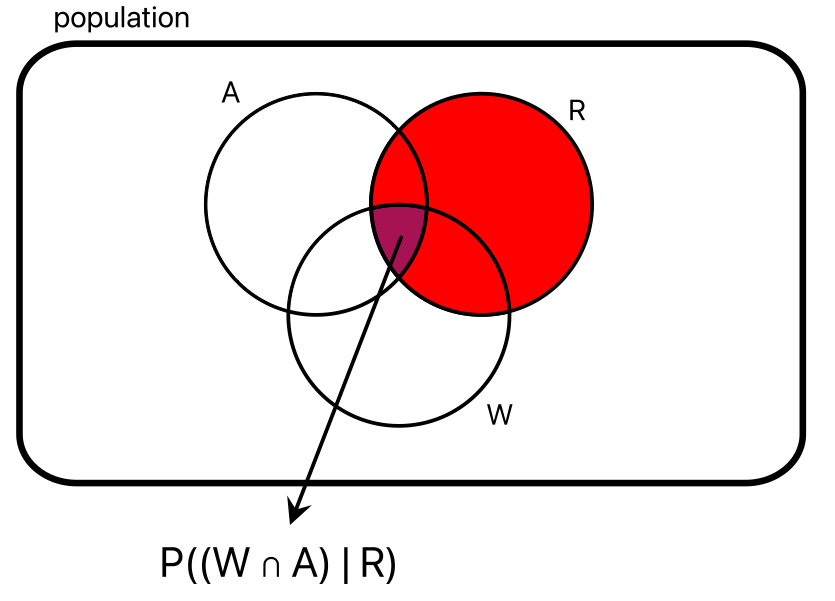
\includegraphics[height=0.4\textheight]{images/set.png}
                    \end{figure}                    
                    
                    \vskip -0.5em
                    {\scriptsize{\begin{alertblock}{Event Reminder}
                        \begin{itemize}
                            \item W = Wants to WFH
                            \item R = Job is remote-ready
                            \item A = Employer allows WFH
                            \item $W_p$ = Wanted to WFH pre-pandemic.
                        \end{itemize}                        
                        \textit{All probabilities for a \textbf{particular} individual worker.}
                    \end{alertblock}}}
                    
                \end{column}
                \begin{column}{0.01\linewidth}
                    
                \end{column}
                
                \begin{column}{0.49\linewidth}
                    \begin{align*}
                        P((W \cap A) | R) & \equiv \pause
                        \frac{P(W \cap A \cap R)}{P(R)} \\[1em]  \pause
                        &\equiv \frac{P(W)\cdot P(A \cap R)}{P(R)} \\[1em]  \pause
                        & \equiv  \frac{c\cdot P(W_p)\cdot P(A \cap R)}{P(R)}\\[1em]  \pause
                        &\equiv  \frac{(1.4)\cdot P(W_p \cap A \cap R)}{P(R)}
                    \end{align*}
            
                \end{column}                
            \end{columns}
            
                        \vskip 0.8em
        \end{frame}
        \begin{frame}{Estimating $P(W_p \cap A \cap R)$ for a Given Worker}
            \begin{columns}
                \begin{column}{0.5\linewidth}
                    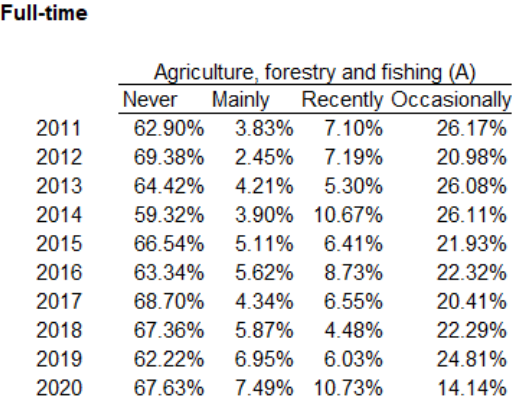
\includegraphics[width=200px]{exampleONSTable.png}
                \end{column}                
                \begin{column}{0.5\linewidth}
                    \begin{equation*}
                        P((W \cap A) | R) \equiv
                        \frac{(1.4)\cdot \tikzmarkin<1>[set fill color=yellow,set border color=yellow]{q}(0,0.4)(0,-0.1) P(W_p \cap A \cap R) \tikzmarkend{q}}{P(R)}
                    \end{equation*}
                        
                \end{column}
            \end{columns}
                
                %
        
            \footnotetext[1]{Homeworking in the UK, work from home status, ONS, 2021}
        \end{frame}
        
        \begin{frame}{Estimating $P(W_p \cap A \cap R)$ for a Given Worker}
            %\textbf{Technical Computing Algorithm Pseudocode}
      %          \begin{columns}[T]
%                    \begin{column}{0.05\linewidth}
 %                   \end{column}
  %                  \begin{column}{0.95\linewidth}
   %                 \lstinputlisting{code/model2Pseudo.c}

    %                \end{column}
     %           \end{columns}
               % \textcolor{navy}{
            
            \vskip -3em               
                \begin{columns}[T]
                    \begin{column}{0.65\linewidth}
                                
                    \end{column}
                    \begin{column}{0.35\linewidth}
                        {\scriptsize \begin{equation*}
                        \boxed{P((W \cap A) | R) \equiv
                            \frac{(1.4)\cdot \tikzmarkin<1->[set fill color=yellow,set border color=yellow]{llll}(0,0.25)(0,-0.05) P(W_p \cap A \cap R) \tikzmarkend{llll}}{P(R)}}
                        \end{equation*}}

                    \end{column}
                \end{columns}
                \vskip 0.5em

                    

               \textbf{Equation Equivalent to the OOP Technical Computing Algorithm}
               \vskip 12 ex
               
               
                \begin{equation*}
                    P(W_p \cap A \cap R)_{est} = 
                    \tikzmarkin<2>[set fill color=white,set border color=navy]{a}(0.05,-0.10)(-0.05,0.35) B \tikzmarkend{a} \cdot \tikzmarkin<3>[set fill color=white, set border color=red]{d}(0,-0.6)(0,0.6) \prod_{char}  \left (  \frac{\alt<3>{ \LabelText<3>{\tikzmarkin<3>[set fill color=white,set border color=navy]{f}(0,-0.1)(0,0.30) ONSRate2019(char)\tikzmarkend{f} }{\scriptsize e.g. 0.2 when char = `Asian' if, in 2019, 20\% of Asians worked from home.}{navy}{8.0ex}}{ONSRate2019(char)}}{B}\right) \tikzmarkend{d} \cdot \alt<4>{\LabelText<4>{\tikzmarkin<4>[set fill color=white,set border color=navy]{b}(0.05,-0.1)(-0.05,0.3) \tanh{(C)} \tikzmarkend{b}}{\scriptsize Commute distance scaling factor.}{navy}{8.0ex}}{\tanh{(C)}} \cdot\alt<5>{\LabelText<5>{\tikzmarkin<5>[set fill color=white,set border color=red]{c}(-0.01,0.5)(0.01,-0.2) \relax (1.5-0.5 \cdot e^{\frac{Y-20}{80}}) \tikzmarkend{c}}{\scriptsize Age scaling factor.}{red}{8.0ex}}{(1.5-0.5 \cdot e^{\frac{Y-20}{80}})}
                \end{equation*}
                 %\tag{$\ddagger$}
                 
                
                % set fill color=yellow,set border color=yellow
                
                \footnotetext[1]{\scriptsize \alt<2>{\colorbox<2>{yellow}{B = 'base' WFH rate for the whole population $\approx 0.266$;}}{B = 'base' WFH rate for the whole population $\approx 0.266$;} C = commute distance; Y = age in years; \\ char = one characteristic of a \textit{particular worker's} demographic, e.g. \textit{their particular} ethnicity or industry.}

        \end{frame}        
        
        \begin{frame}{Problem II Model}
            \begin{equation*}
                P((W \cap A) | R) \approx \frac{c \cdot P(W_p \cap A \cap R)_{est}}{{P(R)}}
            \end{equation*}
            
            
            \footnotetext[1]{$P(R)$ : Remote Work: Fad or Future, M3 Challenge 2022 Dataset, D3}
        \end{frame}
        
    \subsection{Applying \& Evaluating the Model}
        \begin{frame}{Results}
            \scriptsize\begin{table}[h!]
                \begin{center}
                \bgroup
                \def\arraystretch{1.4}%  1 is the default

                \begin{tabular}{|c|c|c|c|c|P{1.6cm}|c|P{1.4cm}|P{1.2cm}|}
                  \hline 
                \textbf{Sex} & \textbf{Ethnicity} & \textbf{Sector} & \textbf{Education} & \textbf{FT/PT} & {\centering {\textbf{Commute Distance, m}}} & \textbf{Age} & \textbf{WFH Probability} & {\centering {\textbf{Effect of change}}} \\ 
                  \hline 
                Male & White & IT & Degree & FT & {\centering 1000} & 40 & 0.63493 & {\centering  -} \\ \hline
                Male & White & IT & Degree & FT & {\centering 1000} & \textcolor{red}{80} & 0.32672 & {\centering $\downarrow$} \\ \hline
                Male & White & IT & \textcolor{red}{No Qualification} & FT & {\centering 1000} & \textcolor{red}{40} & 0.19411 & {\centering $\downarrow$}\\ \hline
                \textcolor{red}{Female} & White & IT & No Qualification & FT & {\centering 1000} & 40 & 0.55491 & {\centering $\uparrow$} \\ \hline
                Female & \textcolor{red}{Asian} & IT & No Qualification & FT & {\centering 1000} & 40 & 0.13247 & {\centering $\downarrow$} \\ \hline
                Female & Asian & \textcolor{red}{Retail} & No Qualification & FT & {\centering 1000} & 40 & 0.17857 & {\centering $\uparrow$} \\ \hline
                Female & Asian & Retail & No Qualification & FT & {\centering \textcolor{red}{400}} & 40 & 0.08909 &  {\centering $\downarrow$} \\ \hline
                Female & Asian & Retail & \textcolor{red}{A Level (High School)} & FT & {\centering 400} & 40 & 0.23094 & {\centering $\uparrow$} \\
                    
                    \hline
                \end{tabular}
\caption{Example work-from-home probabilities for candidates with different characteristics, showing \alert{incremental changes.}}                
                \egroup
            \end{center}
            \end{table}
            \end{frame}
            
\section{Part III: Just a Little Home-work}
    \sectionheader
        \subsection{Problem Statement}
        \begin{frame}{Problem Statement}
        \begin{enumerate}
            \itemsep 1em
            \item Synthesize models from the first two questions to create a model which, for a given city, estimates the percentage of workers who will work remotely. \pause
            \item Apply to Seattle, Omaha, Scranton, Liverpool, and Barry in 2024 and 2027. \pause
            \item Use to relatively rank the different cities by the impact of remote work on them. 
        \end{enumerate}
        
            
        \end{frame}
    \subsection{Assumptions}
        \begin{frame}{Assumptions \& Variables}
            \textbf{Critical Assumption}
            \begin{itemize}
                \item[$\rightarrow$]{Within each sex, each ethnicity is distributed in the same way as it is for the whole population, and so on for other demographic factors and the industries.}
            \end{itemize}
            \vskip 1em \pause
            \textbf{Features \& Variables}
            \begin{itemize}
                \item[$\rightarrow$]{We use the same factors as in the previous two parts, as we combine those models to produce this one.}
            \end{itemize}            
        \end{frame}

    \subsection{Developing the Model}
        \begin{frame}{Developing the Model}
        \pause
            \begin{itemize}
                \itemsep 0.5em
                \item[$\rightarrow$] Part I : city level, proportion of remote ready jobs. \pause
                \item[$\rightarrow$] Part II : individual level, chance of WFH given remote ready. \pause
                \item[$\rightarrow$] Part III : city level, proportion of actual home-workers. \pause
            \end{itemize}
            \vskip 1em
            \textbf{$\therefore$ Population Simulation Method} \pause
            \vskip 1em
            \begin{enumerate}
                \itemsep 0.5em
                \item Part I gives industry sizes each year, each city; other demographic data researched. \pause
                \item Generate representative population of Person objects. \pause
                \item Run each Person through model II; aggregate over the city.
            \end{enumerate}
        \end{frame}
    
    \begin{frame}{The RecursiveGen Procedure : Diagrammatic Representation}
        \textbf{\alt<2>{Repeat for all cities, in 2024 and 2027}{Seattle, 2024}} \\
        

        \begin{tikzpicture}
            \path (-5,0) pic {recurGenDiagram};
        \end{tikzpicture}        
        \footnotetext[1]{Icons from Freepik via Flaticon}
    \end{frame}
      

%    \begin{frame}{Part III Model : The RecursiveGen Procedure : Pseudocode}
%        \vskip-1.3em
%        \begin{columns}[]
%            \begin{column}{0.05\linewidth}
%            \end{column}
%            \begin{column}{0.95\linewidth}
%                \lstinputlisting{code/model3RecursiveGen.c}
%            \end{column}      
%        \end{columns}    
%    \end{frame} 

   % \begin{frame}{Part III Model : Technical Computing Algorithm Pseudocode}
    %    \begin{tikzpicture}
     %   \node[draw,text width=2cm] at (5,0) {For each city};
      %  \node[draw,text width=2cm] at (7,0) {For 2024 and 2027};

       % \path (0,0) pic[scale=0.5] {recurGenDiagram};

        %\end{tikzpicture}

      
      %  \vskip-1.7em

     %   \begin{columns}[T]
%            \begin{column}{0.05\linewidth}
 %           \end{column}
  %          \begin{column}{0.95\linewidth}
   %             \lstinputlisting{code/model3Pseudo.c}
    %        \end{column}      
    
    
    %    \end{columns}
%    \end{frame}             

    \subsection{Applying the Model}
        \begin{frame}{Problem III Results}
                \underline{Actual Work From Home Percentage}
                \begin{table}[h!]
                  \begin{center}
                    \label{tab:resultsFinal} % Use this to create a label for the table so you can later reference it with \ref
                    \begin{tabular}{|c|c|c|c|c|} % Defines where vertical lines appear and the column alignment left centre or right
                      \toprule 
                       \textbf{City} & \textbf{2024 predictions} & \textbf{2024 ranking} & \textbf{2027 predictions} & \textbf{2027 ranking} \\
                      \midrule 
                      Seattle & 30.73\% & 1st & 32.45\% & 1st  \\
                      Omaha & 29.07\% & 2nd & 29.26\% & 2nd  \\
                      Liverpool & 27.37\% & 3rd & 29.13\% & 3rd  \\
                      Barry & 26.51\% & 4th & 26.59\% & \alert{5th}  \\
                      Scranton & 26.36\% & 5th & 26.63\% & \alert{4th}  \\
                      \bottomrule 
                    \end{tabular}
                    %\caption{Summary of Problem III Results for 2024 \& 2027} 
                  \end{center}
                \end{table}
        \end{frame}
        

    \subsection{Evaluating the Model}
        %\begin{frame}{Sensitivity Analysis}
         %       \begin{table}[h!]
          %        \begin{center}
         %           \label{tab:variables1} % Use this to create a label for the table so you can later reference it with \ref
    %                \begin{tabular}{|c|c|c|c|c|c|c|} % Defines where vertical lines appear and the column alignment left centre or right
     %                 \toprule 
                       %\textbf{$\Delta$c} & \textbf{Barry} & %\textbf{Liverpool} & \textbf{Omaha} & \textbf{Seattle} & \textbf{Scranton}& \textbf{Average}\\
                      %\midrule 
                      %+10\% & +9.7\% & +9.8\% & +9.9\% & +9.8\% & +9.7\% & +9.78\%\\
    %                   +5\%  & +4.5\% & +4.9\% & +4.9\% & +4.8\% & +4.6\% & +4.74\% \\ 
%                       -5\% & -4.8\% & -4.7\% & -5.0\% & -4.7\% & -5.1\% & -4.86\%\\
    %                   -10\% & -9.7\% & -10.0\% & -9.9\% & -9.9\% & -9.9\% & -9.88\%\\
                  %    \bottomrule 
                 %   \end{tabular}
                %    \caption{Sensitivity Analysis on the Pandemic Correction Constant for Part III} 
%                  \end{center}
%                \end{table}        
%        \end{frame}
        
    \subsection{Evaluating the Model}
        \begin{frame}{Strengths and Weaknesses} % MAYBE SKIP
            \begin{itemize}
                \item[\textcolor{armygreen}{\textbf{+}}] c.f. post-pandemic estimates $\approx$ 30 \% $\rightarrow$ Slight increase now to 2024/7 as expected. \pause
                \item[\textcolor{armygreen}{\textbf{+}}] Applicable to any city, not just those provided. \pause
                \item[\textcolor{armygreen}{\textbf{+}}] Considers a wide range of factors. 
                \item[\textcolor{armygreen}{\textbf{+}}] Models I, II, III give results consistent with each other.  \pause
                
            \end{itemize}
            \vskip 1em
            \begin{itemize}
                \item[\textcolor{red}{\textbf{---}}] Time-consuming to extend to other cities; lots of data formatting required. \pause
                \item[\textcolor{red}{\textbf{---}}] Pandemic constant (c) has a large impact (see sensitivity analysis). \pause
                \item[\textcolor{red}{\textbf{---}}] Sub-demographic assumption time-saving but not necessarily realistic.       
            \end{itemize}            
        \end{frame}        

%% Do add any more you can think of.
\section{Conclusion and Further Studies}
    \sectionheader
    \begin{frame}{Conclusion and Further Studies}
        \begin{block}{Conclusions}
            \begin{itemize}
                \item<2-> Post-pandemic, remote work will increase between now and 2027 in all cities:\\
                    $\rightarrow$ Avoid disadvantaging remote workers in labour policies.
                \item<3-> Inter-city range in WFH \% will increase: %more
                    \\ $\rightarrow$ Avoid inequality by investing in towns like Barry.
            \end{itemize}
        \end{block}
        \vskip 0.4em
%% Do add any more you can think of.
        \begin{alertblock}{Extending our Work}
            \begin{itemize}
                \item<4-> Assess and reduce impact of Model III assumptions; reduce data dependence.
                \item<5-> Make c individual-dependent (sub-model).
                \item<6-> Explore causes of US vs UK differences in our model.
            \end{itemize}
        \end{alertblock}
        
    \end{frame}

%\begin{frame}
%\frametitle{Sample frame title}

%In this slide, some important text will be
%\alert{highlighted} because it's important.

%\begin{block}{Remark}
%Sample text
%\end{block}

%\begin{alertblock}{Important theorem}
%Sample text in red box
%\end{alertblock}

%\begin{examples}
%Sample text in green box. The title of the block is ``Examples".
%\end{examples}
%\end{frame}


\section{Questions}

    \begin{frame}
    \Huge{\centerline{\textcolor{red}{Thank you!}}}
    \vskip 0.5em
    \large{\centerline{\textcolor{navy}{Any questions?}}}
    \end{frame}



\end{document}